\documentclass{standalone}
\usepackage{tikz}
\usetikzlibrary{patterns, positioning}

\begin{document}
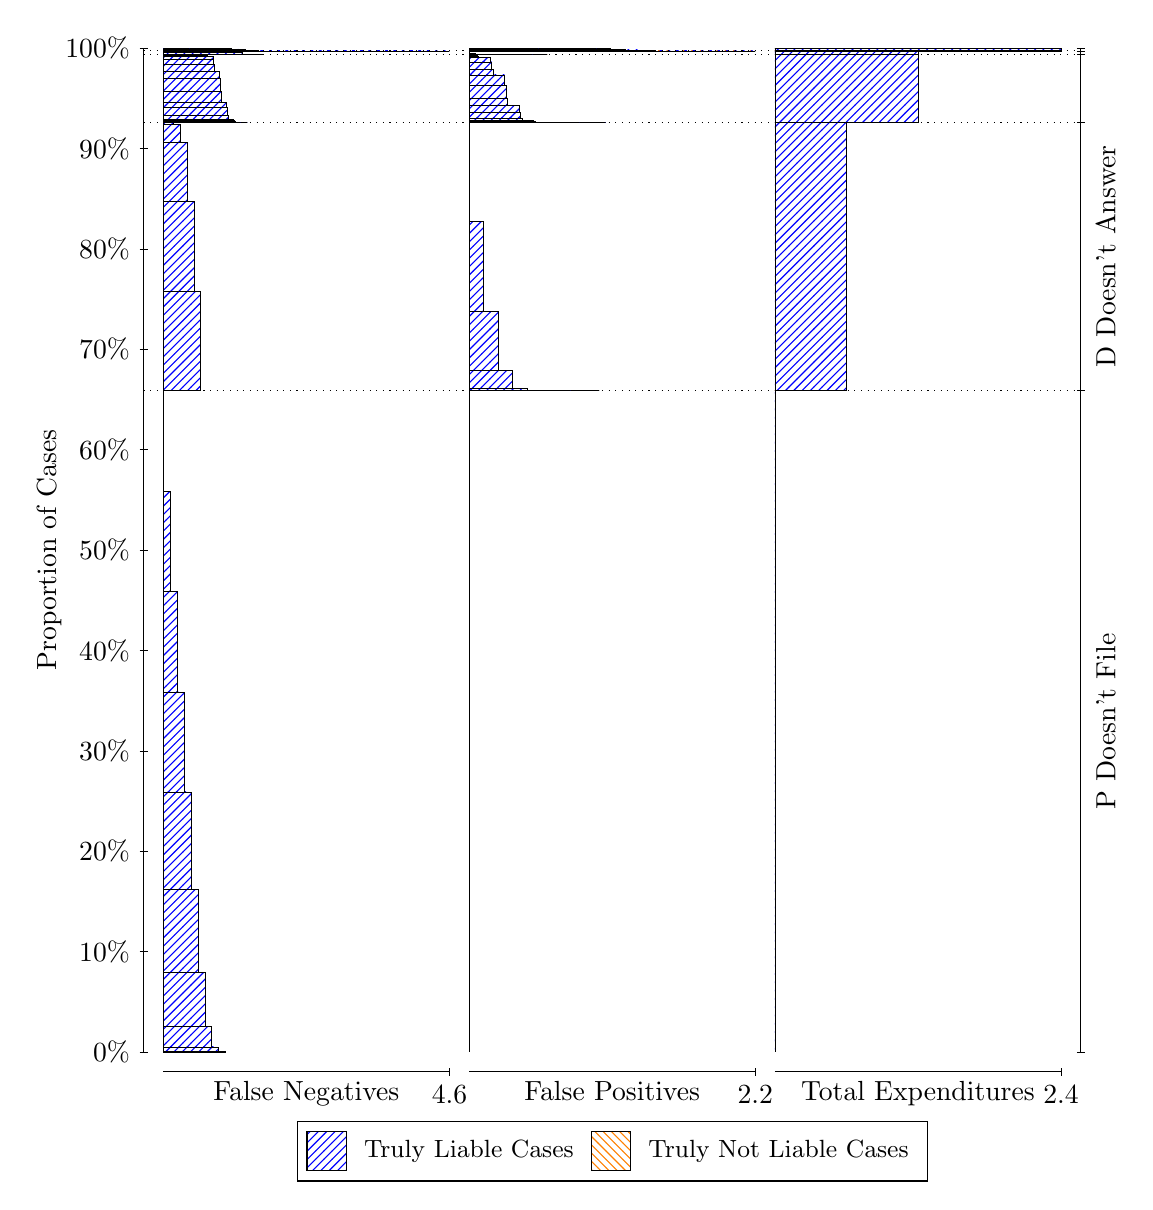
\begin{tikzpicture}
\draw[black, very thin] (1.5,1.75) -- (1.5,14.5);
\node[rotate=90, anchor=center] at (0.3, 8.125) {Proportion of Cases};
\draw[black, very thin] (1.45,1.75) -- (1.55,1.75);
\node[anchor=east] at (1.45, 1.75) {0\%};
\draw[black, very thin] (1.45,3.025) -- (1.55,3.025);
\node[anchor=east] at (1.45, 3.025) {10\%};
\draw[black, very thin] (1.45,4.3) -- (1.55,4.3);
\node[anchor=east] at (1.45, 4.3) {20\%};
\draw[black, very thin] (1.45,5.575) -- (1.55,5.575);
\node[anchor=east] at (1.45, 5.575) {30\%};
\draw[black, very thin] (1.45,6.85) -- (1.55,6.85);
\node[anchor=east] at (1.45, 6.85) {40\%};
\draw[black, very thin] (1.45,8.125) -- (1.55,8.125);
\node[anchor=east] at (1.45, 8.125) {50\%};
\draw[black, very thin] (1.45,9.4) -- (1.55,9.4);
\node[anchor=east] at (1.45, 9.4) {60\%};
\draw[black, very thin] (1.45,10.675) -- (1.55,10.675);
\node[anchor=east] at (1.45, 10.675) {70\%};
\draw[black, very thin] (1.45,11.95) -- (1.55,11.95);
\node[anchor=east] at (1.45, 11.95) {80\%};
\draw[black, very thin] (1.45,13.225) -- (1.55,13.225);
\node[anchor=east] at (1.45, 13.225) {90\%};
\draw[black, very thin] (1.45,14.5) -- (1.55,14.5);
\node[anchor=east] at (1.45, 14.5) {100\%};

\draw[black, very thin] (13.4,1.75) -- (13.4,14.5);
\draw[black, very thin] (13.35,1.75) -- (13.45,1.75);
\node[anchor=west] at (13.35, 1.75) {};
\draw[black, very thin] (13.35,10.149) -- (13.45,10.149);
\node[anchor=west] at (13.35, 10.149) {};
\draw[black, very thin] (13.35,13.557) -- (13.45,13.557);
\node[anchor=west] at (13.35, 13.557) {};
\draw[black, very thin] (13.35,14.415) -- (13.45,14.415);
\node[anchor=west] at (13.35, 14.415) {};
\draw[black, very thin] (13.35,14.464) -- (13.45,14.464);
\node[anchor=west] at (13.35, 14.464) {};
\draw[black, very thin] (13.35,14.5) -- (13.45,14.5);
\node[anchor=west] at (13.35, 14.5) {};

\draw[black, very thin, pattern color=blue, pattern=north east lines] (1.75,1.75) rectangle (2.5399,1.7568);
\draw[black, very thin, pattern color=blue, pattern=north east lines] (1.75,1.7568) rectangle (2.4521,1.8135);
\draw[black, very thin, pattern color=blue, pattern=north east lines] (1.75,1.8135) rectangle (2.3643,2.0796);
\draw[black, very thin, pattern color=blue, pattern=north east lines] (1.75,2.0796) rectangle (2.2766,2.7572);
\draw[black, very thin, pattern color=blue, pattern=north east lines] (1.75,2.7572) rectangle (2.1888,3.8182);
\draw[black, very thin, pattern color=blue, pattern=north east lines] (1.75,3.8182) rectangle (2.101,5.0529);
\draw[black, very thin, pattern color=blue, pattern=north east lines] (1.75,5.0529) rectangle (2.0133,6.3244);
\draw[black, very thin, pattern color=blue, pattern=north east lines] (1.75,6.3244) rectangle (1.9255,7.5993);
\draw[black, very thin, pattern color=blue, pattern=north east lines] (1.75,7.5993) rectangle (1.8378,8.8743);
\draw[black, very thin, pattern color=orange, pattern=north west lines] (1.75,8.8743) rectangle (1.75,8.8743);
\draw[black, very thin, pattern color=blue, pattern=north east lines] (1.75,8.8743) rectangle (1.75,10.149);
\draw[black, very thin, pattern color=blue, pattern=north east lines] (1.75,10.149) rectangle (2.2239,11.408);
\draw[black, very thin, pattern color=blue, pattern=north east lines] (1.75,11.408) rectangle (2.1362,12.556);
\draw[black, very thin, pattern color=blue, pattern=north east lines] (1.75,12.556) rectangle (2.0484,13.301);
\draw[black, very thin, pattern color=blue, pattern=north east lines] (1.75,13.301) rectangle (1.9606,13.532);
\draw[black, very thin, pattern color=blue, pattern=north east lines] (1.75,13.532) rectangle (1.8729,13.556);
\draw[black, very thin, pattern color=blue, pattern=north east lines] (1.75,13.556) rectangle (1.7851,13.557);
\draw[black, very thin, pattern color=orange, pattern=north west lines] (1.75,13.557) rectangle (1.75,13.557);
\draw[black, very thin, pattern color=blue, pattern=north east lines] (1.75,13.557) rectangle (1.75,13.557);
\draw[black, very thin, pattern color=blue, pattern=north east lines] (1.75,13.557) rectangle (2.8163,13.557);
\draw[black, very thin, pattern color=blue, pattern=north east lines] (1.75,13.557) rectangle (2.7373,13.558);
\draw[black, very thin, pattern color=blue, pattern=north east lines] (1.75,13.558) rectangle (2.7285,13.558);
\draw[black, very thin, pattern color=blue, pattern=north east lines] (1.75,13.558) rectangle (2.6583,13.567);
\draw[black, very thin, pattern color=blue, pattern=north east lines] (1.75,13.567) rectangle (2.6496,13.579);
\draw[black, very thin, pattern color=blue, pattern=north east lines] (1.75,13.579) rectangle (2.6408,13.594);
\draw[black, very thin, pattern color=blue, pattern=north east lines] (1.75,13.594) rectangle (2.5706,13.649);
\draw[black, very thin, pattern color=blue, pattern=north east lines] (1.75,13.649) rectangle (2.5618,13.743);
\draw[black, very thin, pattern color=blue, pattern=north east lines] (1.75,13.743) rectangle (2.553,13.813);
\draw[black, very thin, pattern color=blue, pattern=north east lines] (1.75,13.813) rectangle (2.4828,13.946);
\draw[black, very thin, pattern color=blue, pattern=north east lines] (1.75,13.946) rectangle (2.474,14.113);
\draw[black, very thin, pattern color=blue, pattern=north east lines] (1.75,14.113) rectangle (2.4653,14.199);
\draw[black, very thin, pattern color=blue, pattern=north east lines] (1.75,14.199) rectangle (2.395,14.29);
\draw[black, very thin, pattern color=blue, pattern=north east lines] (1.75,14.29) rectangle (2.3863,14.359);
\draw[black, very thin, pattern color=blue, pattern=north east lines] (1.75,14.359) rectangle (2.3775,14.389);
\draw[black, very thin, pattern color=blue, pattern=north east lines] (1.75,14.389) rectangle (2.3073,14.405);
\draw[black, very thin, pattern color=blue, pattern=north east lines] (1.75,14.405) rectangle (2.2985,14.411);
\draw[black, very thin, pattern color=blue, pattern=north east lines] (1.75,14.411) rectangle (2.2897,14.414);
\draw[black, very thin, pattern color=blue, pattern=north east lines] (1.75,14.414) rectangle (2.2195,14.415);
\draw[black, very thin, pattern color=blue, pattern=north east lines] (1.75,14.415) rectangle (2.2107,14.415);
\draw[black, very thin, pattern color=blue, pattern=north east lines] (1.75,14.415) rectangle (2.202,14.415);
\draw[black, very thin, pattern color=blue, pattern=north east lines] (1.75,14.415) rectangle (2.1318,14.415);
\draw[black, very thin, pattern color=blue, pattern=north east lines] (1.75,14.415) rectangle (2.123,14.415);
\draw[black, very thin, pattern color=blue, pattern=north east lines] (1.75,14.415) rectangle (2.1142,14.415);
\draw[black, very thin, pattern color=blue, pattern=north east lines] (1.75,14.415) rectangle (2.044,14.415);
\draw[black, very thin, pattern color=blue, pattern=north east lines] (1.75,14.415) rectangle (2.0352,14.415);
\draw[black, very thin, pattern color=blue, pattern=north east lines] (1.75,14.415) rectangle (2.0264,14.415);
\draw[black, very thin, pattern color=blue, pattern=north east lines] (1.75,14.415) rectangle (1.9562,14.415);
\draw[black, very thin, pattern color=blue, pattern=north east lines] (1.75,14.415) rectangle (1.9475,14.415);
\draw[black, very thin, pattern color=blue, pattern=north east lines] (1.75,14.415) rectangle (1.8685,14.415);
\draw[black, very thin, pattern color=orange, pattern=north west lines] (1.75,14.415) rectangle (1.75,14.415);
\draw[black, very thin, pattern color=blue, pattern=north east lines] (1.75,14.415) rectangle (3.0138,14.415);
\draw[black, very thin, pattern color=blue, pattern=north east lines] (1.75,14.415) rectangle (2.926,14.416);
\draw[black, very thin, pattern color=blue, pattern=north east lines] (1.75,14.416) rectangle (2.8382,14.423);
\draw[black, very thin, pattern color=blue, pattern=north east lines] (1.75,14.423) rectangle (2.7505,14.446);
\draw[black, very thin, pattern color=blue, pattern=north east lines] (1.75,14.446) rectangle (2.6627,14.461);
\draw[black, very thin, pattern color=blue, pattern=north east lines] (1.75,14.461) rectangle (2.575,14.464);
\draw[black, very thin, pattern color=blue, pattern=north east lines] (1.75,14.464) rectangle (2.4872,14.464);
\draw[black, very thin, pattern color=blue, pattern=north east lines] (1.75,14.464) rectangle (2.3994,14.464);
\draw[black, very thin, pattern color=blue, pattern=north east lines] (1.75,14.464) rectangle (2.3117,14.464);
\draw[black, very thin, pattern color=blue, pattern=north east lines] (1.75,14.464) rectangle (2.2239,14.464);
\draw[black, very thin, pattern color=orange, pattern=north west lines] (1.75,14.464) rectangle (1.75,14.464);
\draw[black, very thin, pattern color=blue, pattern=north east lines] (1.75,14.464) rectangle (5.3833,14.464);
\draw[black, very thin, pattern color=blue, pattern=north east lines] (1.75,14.464) rectangle (5.2956,14.464);
\draw[black, very thin, pattern color=blue, pattern=north east lines] (1.75,14.464) rectangle (5.2078,14.464);
\draw[black, very thin, pattern color=blue, pattern=north east lines] (1.75,14.464) rectangle (5.12,14.464);
\draw[black, very thin, pattern color=blue, pattern=north east lines] (1.75,14.464) rectangle (5.12,14.464);
\draw[black, very thin, pattern color=blue, pattern=north east lines] (1.75,14.464) rectangle (5.0323,14.464);
\draw[black, very thin, pattern color=blue, pattern=north east lines] (1.75,14.464) rectangle (4.9445,14.464);
\draw[black, very thin, pattern color=blue, pattern=north east lines] (1.75,14.464) rectangle (4.8568,14.464);
\draw[black, very thin, pattern color=blue, pattern=north east lines] (1.75,14.464) rectangle (4.8568,14.464);
\draw[black, very thin, pattern color=blue, pattern=north east lines] (1.75,14.464) rectangle (4.769,14.464);
\draw[black, very thin, pattern color=blue, pattern=north east lines] (1.75,14.464) rectangle (4.6812,14.464);
\draw[black, very thin, pattern color=blue, pattern=north east lines] (1.75,14.464) rectangle (4.5935,14.464);
\draw[black, very thin, pattern color=blue, pattern=north east lines] (1.75,14.464) rectangle (4.5057,14.464);
\draw[black, very thin, pattern color=blue, pattern=north east lines] (1.75,14.464) rectangle (4.418,14.464);
\draw[black, very thin, pattern color=blue, pattern=north east lines] (1.75,14.464) rectangle (3.2244,14.464);
\draw[black, very thin, pattern color=blue, pattern=north east lines] (1.75,14.464) rectangle (3.1366,14.464);
\draw[black, very thin, pattern color=blue, pattern=north east lines] (1.75,14.464) rectangle (3.0489,14.465);
\draw[black, very thin, pattern color=blue, pattern=north east lines] (1.75,14.465) rectangle (2.9611,14.466);
\draw[black, very thin, pattern color=blue, pattern=north east lines] (1.75,14.466) rectangle (2.8733,14.466);
\draw[black, very thin, pattern color=blue, pattern=north east lines] (1.75,14.466) rectangle (2.8733,14.47);
\draw[black, very thin, pattern color=blue, pattern=north east lines] (1.75,14.47) rectangle (2.7856,14.474);
\draw[black, very thin, pattern color=blue, pattern=north east lines] (1.75,14.474) rectangle (2.7856,14.478);
\draw[black, very thin, pattern color=blue, pattern=north east lines] (1.75,14.478) rectangle (2.6978,14.488);
\draw[black, very thin, pattern color=blue, pattern=north east lines] (1.75,14.488) rectangle (2.6101,14.491);
\draw[black, very thin, pattern color=blue, pattern=north east lines] (1.75,14.491) rectangle (2.6101,14.495);
\draw[black, very thin, pattern color=blue, pattern=north east lines] (1.75,14.495) rectangle (2.5223,14.495);
\draw[black, very thin, pattern color=blue, pattern=north east lines] (1.75,14.495) rectangle (2.5223,14.499);
\draw[black, very thin, pattern color=blue, pattern=north east lines] (1.75,14.499) rectangle (2.5223,14.499);
\draw[black, very thin, pattern color=blue, pattern=north east lines] (1.75,14.499) rectangle (2.4345,14.499);
\draw[black, very thin, pattern color=blue, pattern=north east lines] (1.75,14.499) rectangle (2.4345,14.5);
\draw[black, very thin, pattern color=blue, pattern=north east lines] (1.75,14.5) rectangle (2.3468,14.5);
\draw[black, very thin, pattern color=blue, pattern=north east lines] (1.75,14.5) rectangle (2.259,14.5);
\draw[black, very thin, pattern color=blue, pattern=north east lines] (1.75,14.5) rectangle (2.1713,14.5);
\draw[black, very thin, pattern color=blue, pattern=north east lines] (1.75,14.5) rectangle (2.1713,14.5);
\draw[black, very thin, pattern color=blue, pattern=north east lines] (1.75,14.5) rectangle (2.0835,14.5);
\draw[black, very thin, pattern color=blue, pattern=north east lines] (1.75,14.5) rectangle (2.0835,14.5);
\draw[black, very thin, pattern color=blue, pattern=north east lines] (1.75,14.5) rectangle (1.9957,14.5);
\draw[black, very thin, pattern color=blue, pattern=north east lines] (1.75,14.5) rectangle (1.9957,14.5);
\draw[black, very thin, pattern color=blue, pattern=north east lines] (1.75,14.5) rectangle (1.908,14.5);
\draw[black, very thin, pattern color=orange, pattern=north west lines] (1.75,14.5) rectangle (1.75,14.5);
\draw[black, very thin, pattern color=orange, pattern=north west lines] (5.6333,1.75) rectangle (5.6333,1.75);
\draw[black, very thin, pattern color=blue, pattern=north east lines] (5.6333,1.75) rectangle (5.6333,10.149);
\draw[black, very thin, pattern color=orange, pattern=north west lines] (5.6333,10.149) rectangle (7.2848,10.149);
\draw[black, very thin, pattern color=blue, pattern=north east lines] (5.6333,10.149) rectangle (7.2848,10.149);
\draw[black, very thin, pattern color=blue, pattern=north east lines] (5.6333,10.149) rectangle (7.1013,10.149);
\draw[black, very thin, pattern color=blue, pattern=north east lines] (5.6333,10.149) rectangle (6.9178,10.149);
\draw[black, very thin, pattern color=blue, pattern=north east lines] (5.6333,10.149) rectangle (6.7343,10.149);
\draw[black, very thin, pattern color=blue, pattern=north east lines] (5.6333,10.149) rectangle (6.5508,10.15);
\draw[black, very thin, pattern color=blue, pattern=north east lines] (5.6333,10.15) rectangle (6.3673,10.175);
\draw[black, very thin, pattern color=blue, pattern=north east lines] (5.6333,10.175) rectangle (6.1838,10.405);
\draw[black, very thin, pattern color=blue, pattern=north east lines] (5.6333,10.405) rectangle (6.0003,11.151);
\draw[black, very thin, pattern color=blue, pattern=north east lines] (5.6333,11.151) rectangle (5.8168,12.298);
\draw[black, very thin, pattern color=blue, pattern=north east lines] (5.6333,12.298) rectangle (5.6333,13.557);
\draw[black, very thin, pattern color=orange, pattern=north west lines] (5.6333,13.557) rectangle (7.3674,13.557);
\draw[black, very thin, pattern color=blue, pattern=north east lines] (5.6333,13.557) rectangle (7.3674,13.557);
\draw[black, very thin, pattern color=orange, pattern=north west lines] (5.6333,13.557) rectangle (7.2023,13.557);
\draw[black, very thin, pattern color=blue, pattern=north east lines] (5.6333,13.557) rectangle (7.2023,13.557);
\draw[black, very thin, pattern color=blue, pattern=north east lines] (5.6333,13.557) rectangle (7.1839,13.557);
\draw[black, very thin, pattern color=orange, pattern=north west lines] (5.6333,13.557) rectangle (7.0371,13.557);
\draw[black, very thin, pattern color=blue, pattern=north east lines] (5.6333,13.557) rectangle (7.0371,13.557);
\draw[black, very thin, pattern color=blue, pattern=north east lines] (5.6333,13.557) rectangle (7.0188,13.557);
\draw[black, very thin, pattern color=blue, pattern=north east lines] (5.6333,13.557) rectangle (7.0004,13.557);
\draw[black, very thin, pattern color=blue, pattern=north east lines] (5.6333,13.557) rectangle (6.8536,13.557);
\draw[black, very thin, pattern color=blue, pattern=north east lines] (5.6333,13.557) rectangle (6.8353,13.557);
\draw[black, very thin, pattern color=blue, pattern=north east lines] (5.6333,13.557) rectangle (6.8169,13.557);
\draw[black, very thin, pattern color=blue, pattern=north east lines] (5.6333,13.557) rectangle (6.6701,13.557);
\draw[black, very thin, pattern color=blue, pattern=north east lines] (5.6333,13.557) rectangle (6.6518,13.557);
\draw[black, very thin, pattern color=blue, pattern=north east lines] (5.6333,13.557) rectangle (6.6334,13.558);
\draw[black, very thin, pattern color=blue, pattern=north east lines] (5.6333,13.558) rectangle (6.4866,13.561);
\draw[black, very thin, pattern color=blue, pattern=north east lines] (5.6333,13.561) rectangle (6.4683,13.568);
\draw[black, very thin, pattern color=blue, pattern=north east lines] (5.6333,13.568) rectangle (6.4499,13.583);
\draw[black, very thin, pattern color=blue, pattern=north east lines] (5.6333,13.583) rectangle (6.3031,13.613);
\draw[black, very thin, pattern color=blue, pattern=north east lines] (5.6333,13.613) rectangle (6.2848,13.682);
\draw[black, very thin, pattern color=blue, pattern=north east lines] (5.6333,13.682) rectangle (6.2664,13.774);
\draw[black, very thin, pattern color=blue, pattern=north east lines] (5.6333,13.774) rectangle (6.1196,13.859);
\draw[black, very thin, pattern color=blue, pattern=north east lines] (5.6333,13.859) rectangle (6.1013,14.026);
\draw[black, very thin, pattern color=blue, pattern=north east lines] (5.6333,14.026) rectangle (6.0829,14.159);
\draw[black, very thin, pattern color=blue, pattern=north east lines] (5.6333,14.159) rectangle (5.9361,14.229);
\draw[black, very thin, pattern color=blue, pattern=north east lines] (5.6333,14.229) rectangle (5.9178,14.324);
\draw[black, very thin, pattern color=blue, pattern=north east lines] (5.6333,14.324) rectangle (5.8994,14.378);
\draw[black, very thin, pattern color=blue, pattern=north east lines] (5.6333,14.378) rectangle (5.7526,14.393);
\draw[black, very thin, pattern color=blue, pattern=north east lines] (5.6333,14.393) rectangle (5.7343,14.406);
\draw[black, very thin, pattern color=blue, pattern=north east lines] (5.6333,14.406) rectangle (5.7159,14.414);
\draw[black, very thin, pattern color=blue, pattern=north east lines] (5.6333,14.414) rectangle (5.6333,14.415);
\draw[black, very thin, pattern color=orange, pattern=north west lines] (5.6333,14.415) rectangle (6.6242,14.415);
\draw[black, very thin, pattern color=blue, pattern=north east lines] (5.6333,14.415) rectangle (6.6242,14.415);
\draw[black, very thin, pattern color=blue, pattern=north east lines] (5.6333,14.415) rectangle (6.4407,14.415);
\draw[black, very thin, pattern color=blue, pattern=north east lines] (5.6333,14.415) rectangle (6.2572,14.415);
\draw[black, very thin, pattern color=blue, pattern=north east lines] (5.6333,14.415) rectangle (6.0737,14.415);
\draw[black, very thin, pattern color=blue, pattern=north east lines] (5.6333,14.415) rectangle (5.8902,14.418);
\draw[black, very thin, pattern color=blue, pattern=north east lines] (5.6333,14.418) rectangle (5.7067,14.434);
\draw[black, very thin, pattern color=blue, pattern=north east lines] (5.6333,14.434) rectangle (5.6333,14.464);
\draw[black, very thin, pattern color=orange, pattern=north west lines] (5.6333,14.464) rectangle (9.2667,14.464);
\draw[black, very thin, pattern color=blue, pattern=north east lines] (5.6333,14.464) rectangle (9.2667,14.464);
\draw[black, very thin, pattern color=blue, pattern=north east lines] (5.6333,14.464) rectangle (9.0832,14.464);
\draw[black, very thin, pattern color=orange, pattern=north west lines] (5.6333,14.464) rectangle (9.0832,14.464);
\draw[black, very thin, pattern color=blue, pattern=north east lines] (5.6333,14.464) rectangle (9.0832,14.464);
\draw[black, very thin, pattern color=orange, pattern=north west lines] (5.6333,14.464) rectangle (8.8997,14.464);
\draw[black, very thin, pattern color=blue, pattern=north east lines] (5.6333,14.464) rectangle (8.8997,14.464);
\draw[black, very thin, pattern color=blue, pattern=north east lines] (5.6333,14.464) rectangle (8.8997,14.464);
\draw[black, very thin, pattern color=blue, pattern=north east lines] (5.6333,14.464) rectangle (8.7162,14.464);
\draw[black, very thin, pattern color=orange, pattern=north west lines] (5.6333,14.464) rectangle (8.7162,14.464);
\draw[black, very thin, pattern color=blue, pattern=north east lines] (5.6333,14.464) rectangle (8.7162,14.464);
\draw[black, very thin, pattern color=blue, pattern=north east lines] (5.6333,14.464) rectangle (8.7162,14.464);
\draw[black, very thin, pattern color=blue, pattern=north east lines] (5.6333,14.464) rectangle (8.5327,14.464);
\draw[black, very thin, pattern color=orange, pattern=north west lines] (5.6333,14.464) rectangle (8.5327,14.464);
\draw[black, very thin, pattern color=blue, pattern=north east lines] (5.6333,14.464) rectangle (8.5327,14.464);
\draw[black, very thin, pattern color=blue, pattern=north east lines] (5.6333,14.464) rectangle (8.5327,14.464);
\draw[black, very thin, pattern color=blue, pattern=north east lines] (5.6333,14.464) rectangle (8.3492,14.464);
\draw[black, very thin, pattern color=orange, pattern=north west lines] (5.6333,14.464) rectangle (8.3492,14.464);
\draw[black, very thin, pattern color=blue, pattern=north east lines] (5.6333,14.464) rectangle (8.3492,14.464);
\draw[black, very thin, pattern color=blue, pattern=north east lines] (5.6333,14.464) rectangle (8.3492,14.464);
\draw[black, very thin, pattern color=blue, pattern=north east lines] (5.6333,14.464) rectangle (8.1657,14.465);
\draw[black, very thin, pattern color=blue, pattern=north east lines] (5.6333,14.465) rectangle (8.1657,14.465);
\draw[black, very thin, pattern color=orange, pattern=north west lines] (5.6333,14.465) rectangle (8.1657,14.465);
\draw[black, very thin, pattern color=blue, pattern=north east lines] (5.6333,14.465) rectangle (8.1657,14.465);
\draw[black, very thin, pattern color=blue, pattern=north east lines] (5.6333,14.465) rectangle (8.1657,14.465);
\draw[black, very thin, pattern color=blue, pattern=north east lines] (5.6333,14.465) rectangle (7.9822,14.466);
\draw[black, very thin, pattern color=blue, pattern=north east lines] (5.6333,14.466) rectangle (7.9822,14.467);
\draw[black, very thin, pattern color=blue, pattern=north east lines] (5.6333,14.467) rectangle (7.9822,14.469);
\draw[black, very thin, pattern color=blue, pattern=north east lines] (5.6333,14.469) rectangle (7.7987,14.473);
\draw[black, very thin, pattern color=blue, pattern=north east lines] (5.6333,14.473) rectangle (7.7987,14.473);
\draw[black, very thin, pattern color=blue, pattern=north east lines] (5.6333,14.473) rectangle (7.7987,14.476);
\draw[black, very thin, pattern color=blue, pattern=north east lines] (5.6333,14.476) rectangle (7.6152,14.484);
\draw[black, very thin, pattern color=blue, pattern=north east lines] (5.6333,14.484) rectangle (7.6152,14.485);
\draw[black, very thin, pattern color=blue, pattern=north east lines] (5.6333,14.485) rectangle (7.6152,14.486);
\draw[black, very thin, pattern color=blue, pattern=north east lines] (5.6333,14.486) rectangle (7.4316,14.493);
\draw[black, very thin, pattern color=blue, pattern=north east lines] (5.6333,14.493) rectangle (7.4316,14.494);
\draw[black, very thin, pattern color=blue, pattern=north east lines] (5.6333,14.494) rectangle (7.4316,14.494);
\draw[black, very thin, pattern color=blue, pattern=north east lines] (5.6333,14.494) rectangle (7.2481,14.494);
\draw[black, very thin, pattern color=blue, pattern=north east lines] (5.6333,14.494) rectangle (7.2481,14.498);
\draw[black, very thin, pattern color=blue, pattern=north east lines] (5.6333,14.498) rectangle (7.2481,14.498);
\draw[black, very thin, pattern color=blue, pattern=north east lines] (5.6333,14.498) rectangle (7.0646,14.498);
\draw[black, very thin, pattern color=blue, pattern=north east lines] (5.6333,14.498) rectangle (7.0646,14.499);
\draw[black, very thin, pattern color=blue, pattern=north east lines] (5.6333,14.499) rectangle (6.8811,14.499);
\draw[black, very thin, pattern color=blue, pattern=north east lines] (5.6333,14.499) rectangle (6.8811,14.5);
\draw[black, very thin, pattern color=blue, pattern=north east lines] (5.6333,14.5) rectangle (6.6976,14.5);
\draw[black, very thin, pattern color=blue, pattern=north east lines] (5.6333,14.5) rectangle (6.5141,14.5);
\draw[black, very thin, pattern color=orange, pattern=north west lines] (5.6333,14.5) rectangle (5.6333,14.5);
\draw[black, very thin, pattern color=blue, pattern=north east lines] (5.6333,14.5) rectangle (5.6333,14.5);
\draw[black, very thin, pattern color=orange, pattern=north west lines] (9.5167,1.75) rectangle (9.5167,1.75);
\draw[black, very thin, pattern color=blue, pattern=north east lines] (9.5167,1.75) rectangle (9.5167,10.149);
\draw[black, very thin, pattern color=orange, pattern=north west lines] (9.5167,10.149) rectangle (10.425,10.149);
\draw[black, very thin, pattern color=blue, pattern=north east lines] (9.5167,10.149) rectangle (10.425,13.557);
\draw[black, very thin, pattern color=orange, pattern=north west lines] (9.5167,13.557) rectangle (11.333,13.557);
\draw[black, very thin, pattern color=blue, pattern=north east lines] (9.5167,13.557) rectangle (11.333,14.415);
\draw[black, very thin, pattern color=orange, pattern=north west lines] (9.5167,14.415) rectangle (11.333,14.415);
\draw[black, very thin, pattern color=blue, pattern=north east lines] (9.5167,14.415) rectangle (11.333,14.464);
\draw[black, very thin, pattern color=orange, pattern=north west lines] (9.5167,14.464) rectangle (13.15,14.464);
\draw[black, very thin, pattern color=blue, pattern=north east lines] (9.5167,14.464) rectangle (13.15,14.467);
\draw[black, very thin, pattern color=orange, pattern=north west lines] (9.5167,14.467) rectangle (13.15,14.467);
\draw[black, very thin, pattern color=blue, pattern=north east lines] (9.5167,14.467) rectangle (13.15,14.494);
\draw[black, very thin, pattern color=orange, pattern=north west lines] (9.5167,14.494) rectangle (13.15,14.494);
\draw[black, very thin, pattern color=blue, pattern=north east lines] (9.5167,14.494) rectangle (13.15,14.5);
\draw[black, dotted] (1.5,10.149) -- (13.4,10.149);
\draw[black, dotted] (1.5,13.557) -- (13.4,13.557);
\draw[black, dotted] (1.5,14.415) -- (13.4,14.415);
\draw[black, dotted] (1.5,14.464) -- (13.4,14.464);
\draw[black, very thin] (1.75,1.5) -- (5.3833,1.5);
\node[anchor=north] at (3.5667, 1.5) {False Negatives};
\draw[black, very thin] (5.3833,1.45) -- (5.3833,1.55);
\node[anchor=north] at (5.3833, 1.45) {4.6};

\draw[black, very thin] (5.6333,1.5) -- (9.2667,1.5);
\node[anchor=north] at (7.45, 1.5) {False Positives};
\draw[black, very thin] (9.2667,1.45) -- (9.2667,1.55);
\node[anchor=north] at (9.2667, 1.45) {2.2};

\draw[black, very thin] (9.5167,1.5) -- (13.15,1.5);
\node[anchor=north] at (11.333, 1.5) {Total Expenditures};
\draw[black, very thin] (13.15,1.45) -- (13.15,1.55);
\node[anchor=north] at (13.15, 1.45) {2.4};

\node[black, centered, rotate=90] at (13.72, 5.9497) {P Doesn't File};
\node[black, centered, rotate=90] at (13.72, 11.853) {D Doesn't Answer};




\draw (7.449999999999999,1.5) node[draw=none] (baseCoordinate) {};
\begin{scope}[align=center]
        \matrix[scale=0.5, draw=black, below=0.5cm of baseCoordinate, nodes={draw}, column sep=0.1cm]{
            \node[rectangle, draw, minimum width=0.5cm, minimum height=0.5cm, pattern=north east lines, pattern color=blue] {}; &
            \node[draw=none, font=\small] (B) {Truly Liable Cases}; &
            \node[rectangle, draw, minimum width=0.5cm, minimum height=0.5cm, pattern=north west lines, pattern color=orange] {}; &
            \node[draw=none, font=\small] (B) {Truly Not Liable Cases}; \\
            };
\end{scope}

\end{tikzpicture}
\end{document}